\documentclass[conference]{IEEEtran}
\pagestyle{plain}
\usepackage[pdftex]{graphicx}
\graphicspath{{../pdf/}{../jpeg/}}
\DeclareGraphicsExtensions{.pdf,.jpeg,.png}
\usepackage{changepage}
\usepackage[utf8]{inputenc}
\usepackage[T1]{fontenc}
\usepackage{matlab-prettifier}
%\usepackage[english, spanish]{babel}
\usepackage{circuitikz, siunitx}
\usepackage[cmex10]{amsmath}
\usepackage{mathabx}
\usepackage{algorithmic}
\usepackage{float}
\usepackage{array}
\usepackage{mdwmath}
\usepackage{mdwtab}
\usepackage{eqparbox}
\usepackage{url}
\usepackage{makecell}
\usepackage{tikz}
\usepackage{xcolor}
\IEEEoverridecommandlockouts
\IEEEpeerreviewmaketitle

\usetikzlibrary{shapes.geometric, arrows, arrows.meta, positioning, patterns}

\tikzstyle{startstop} = [rectangle, rounded corners, 
minimum width=3cm, 
minimum height=1cm,
text centered, 
draw=black]

\tikzstyle{io} = [trapezium, 
trapezium stretches=true, % A later addition
trapezium left angle=70, 
trapezium right angle=110, 
minimum width=3cm, 
minimum height=1cm, text centered, 
draw=black]

\tikzstyle{process} = [rectangle, 
minimum width=3cm, 
minimum height=1cm, 
text centered, 
text width=3cm, 
draw=black]

\tikzstyle{decision} = [diamond, 
minimum width=3cm, 
minimum height=1cm, 
text centered, 
draw=black]

\tikzstyle{arrow} = [thick,->,>=stealth]
\tikzstyle{invarrow} = [thick,<-,>=stealth]
        
\begin{document}

\title{Diseño e implementación de un sensor optoelectrónico para la detección y clasificación de colores mediante reflectancia usando ESP32.\\ {\huge Design and Implementation Optoelectronic Sensor for Color Detection and Classification via Reflectance using ESP32.}}

\author{
    \authorblockN{
        M. Rodríguez \\
    }
    \authorblockA{
        \textit{Universidad de los Llanos} \\
        \textit{Villavicencio, Colombia} \\ 
        {\small \texttt{marodriguez.payares@unillanos.edu.co 161004834}}
    }
}
\IEEEaftertitletext{\vspace{-1\baselineskip}}
\maketitle

\renewcommand\abstractname{Resumen}
\begin{abstract}
El presente documento describe el diseño, montaje y calibración de un sistema optoelectrónico capaz de detectar y diferenciar múltiples tarjetas de colores. El sistema utiliza un microcontrolador ESP32, un diodo emisor de luz (LED) RGB y un fotorresistor (LDR). El principio de funcionamiento se basa en la reflectancia de la luz \cite{ldr_2}: el LED RGB ilumina secuencialmente la superficie de prueba con luz roja, verde y azul, mientras que el LDR mide la intensidad de la luz reflejada para cada longitud de onda \cite{ldr_3}. Mediante el uso de un entorno ópticamente aislado y un algoritmo de calibración \cite{ldr_4}, el ESP32 lee las variaciones analógicas generadas en un circuito divisor de tensión para asignar una firma espectral única a cada color. Los resultados demuestran que este enfoque es un método eficaz, escalable y de bajo costo para la clasificación de superficies coloreadas en entornos controlados.
\end{abstract}

\renewcommand\IEEEkeywordsname{Palabras clave}
\begin{keywords}
ESP32, Fotorresistor (LDR), LED RGB, Sensor de color, Reflectancia, Optoelectrónica, Divisor de tensión.
\end{keywords}

\renewcommand\abstractname{Abstract}
\begin{abstract}
This document describes the design, assembly, and calibration of an optoelectronic system capable of detecting and differentiating multiple colored cards. The system uses an ESP32 microcontroller, an RGB light-emitting diode (LED), and a photoresistor (LDR). The operating principle is based on light reflectance \cite{ldr_2}: the RGB LED sequentially illuminates the test surface with red, green, and blue light, while the LDR measures the intensity of the reflected light for each wavelength \cite{ldr_3}. By utilizing an optically isolated environment and a calibration algorithm \cite{ldr_4}, the ESP32 reads the analog variations generated in a voltage divider circuit to assign a unique spectral signature to each color. The results demonstrate that this approach is an effective, scalable, and low-cost method for classifying colored surfaces in controlled environments.
\end{abstract}

\renewcommand\IEEEkeywordsname{Keywords}
\begin{keywords}
ESP32, Photoresistor (LDR), RGB LED, Color sensor, Reflectance, Optoelectronics, Voltage divider.
\end{keywords}

\section{Introducción}

\subsection{El Sensor LDR: Concepto y Funcionamiento}
Un fotorresistor o LDR (del inglés \textit{Light Dependent Resistor}) es un componente electrónico pasivo cuya resistencia eléctrica varía en función de la intensidad de la luz que incide sobre su superficie. Están fabricados con materiales semiconductores de alta resistencia, como el sulfuro de cadmio (CdS) \cite{ldr_5}. 

En la oscuridad, el material semiconductor apenas contiene electrones libres, lo que resulta en una resistencia muy alta (a menudo en el rango de los megaohmios, $\text{M}\Omega$). Sin embargo, cuando los fotones de luz impactan el semiconductor, transfieren suficiente energía a los electrones para que salten a la banda de conducción. Esto disminuye drásticamente la resistencia del componente (cayendo a unos pocos cientos de ohmios a plena luz) \cite{ldr_6}.

\begin{figure}[htbp]
    \centering
    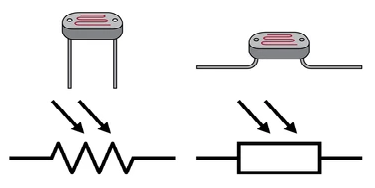
\includegraphics[width=1\linewidth]{ldr.png}
    \caption{Simbología electrónica de un sensor LDR \cite{ldr_1}.}
    \label{fig:ldr}
\end{figure}

\subsection{Ecuación y Curva Característica del LDR}
La relación entre la resistencia del LDR ($R$) y la iluminancia ($E$, medida en lux) no es lineal, sino que sigue una ley de potencia inversa empírica \cite{ldr_7}, expresada matemáticamente como:

\begin{equation}
R = R_0 E^{-\gamma}
\label{eq:caracteristica}
\end{equation}

Donde:
\begin{itemize}
    \item $R$ es la resistencia del LDR para una iluminancia dada.
    \item $R_0$ es la resistencia de calibración a una iluminancia estándar (usualmente $\SI{1}{lux}$).
    \item $E$ es la iluminancia incidente en lux.
    \item $\gamma$ es una constante característica del material (generalmente entre $0.7$ y $0.9$).
\end{itemize}

Esta relación no lineal significa que el LDR es extremadamente sensible a cambios de luz en ambientes oscuros, pero su sensibilidad disminuye en ambientes muy iluminados \cite{ldr_8}.

% Código TikZ para la curva característica
\begin{figure}[htbp]
    \centering
    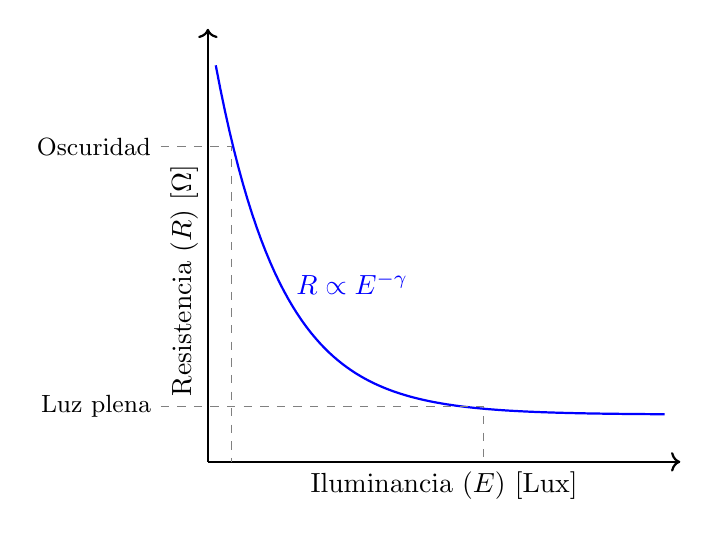
\begin{tikzpicture}[scale=1]
        % Ejes
        \draw[->, thick] (0,0) -- (6,0) node[midway, anchor=north] {Iluminancia ($E$) [Lux]};
        \draw[->, thick] (0,0) -- (0,5.5) node[rotate=90, anchor=east, yshift=0.3cm, xshift=-1.6cm] {Resistencia ($R$) [$\Omega$]};
        
        % Curva característica (exponencial decreciente simulada)
        \draw[thick, blue, domain=0.1:5.8, samples=100] plot (\x, {5*exp(-1.2*\x) + 0.6});
        
        % Etiquetas y puntos guía
        \node[blue, anchor=south west] at (1, 2) {$R \propto E^{-\gamma}$};
        
        % Líneas discontinuas de ejemplo
        \draw[dashed, gray] (-0.6,4) node[anchor=east, text=black]{\small Oscuridad} -- (0.3,4) -- (0.3,0);
        \draw[dashed, gray] (-0.6,0.7) node[anchor=east, text=black]{\small Luz plena} -- (3.5,0.7) -- (3.5,0);
        
    \end{tikzpicture}
    \caption{Curva característica típica de un LDR, mostrando la relación no lineal inversamente proporcional entre la resistencia y la iluminancia.}
    \label{fig:curva_ldr}
\end{figure}

\subsection{El Principio de Reflectancia}
El principio de reflectancia es la base fundamental del sensor de color diseñado en esta práctica. Cuando la luz incide sobre un objeto, ocurren tres fenómenos físicos principales: transmisión, absorción y reflexión. En superficies opacas (como las tarjetas de color), la transmisión es nula \cite{ldr_9}. 

La reflectancia ($R_\lambda$) se define como la fracción de energía luminosa incidente que es reflejada por una superficie, en función de la longitud de onda ($\lambda$) \cite{ldr_10}:

\begin{equation}
R_\lambda = \frac{I_r(\lambda)}{I_0(\lambda)}
\label{eq:reflectancia}
\end{equation}

Donde $I_r$ es la intensidad de la luz reflejada e $I_0$ es la intensidad de la luz incidente.

El color que percibimos de un objeto está determinado por las longitudes de onda que este refleja. Por ejemplo, una tarjeta roja absorbe casi en su totalidad las longitudes de onda correspondientes al azul y al verde, y refleja la longitud de onda del rojo \cite{ldr_11}. Al iluminar secuencialmente la tarjeta con luz pura Roja, Verde y Azul desde el LED RGB, y medir la cantidad de luz que rebota mediante el LDR, podemos construir una "firma espectral" discreta (un vector de tres valores de reflectancia) que identifica unívocamente el color de la tarjeta como se muestra en la figura \ref{fig:principio_reflectancia}.

\begin{figure}[htbp]
    \centering
    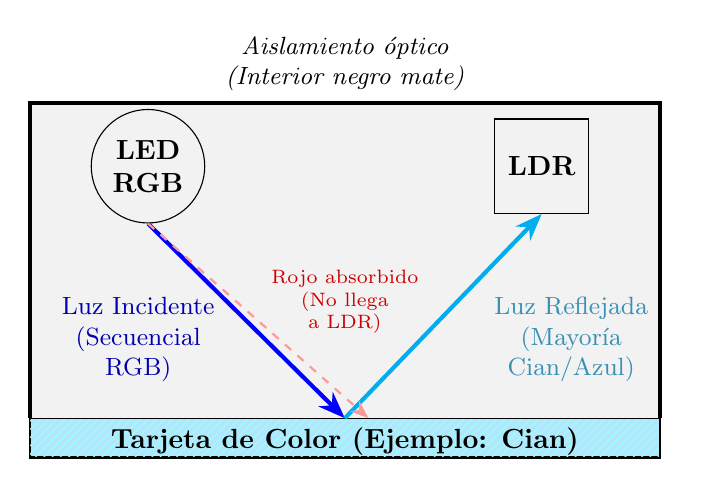
\begin{tikzpicture}[
        node distance = 1cm and 2cm,
        % Estilo para los rayos de luz
        ray/.style={->, >=Stealth, thick},
    ]
        % 1. La Tarjeta de Color (Superficie objetivo)
        % Dibujamos una superficie cian como ejemplo (Cian refleja Verde y Azul, absorbe Rojo)
        \draw[fill=cyan!30, thick] (-4,0) rectangle (4,-0.5);
        \draw[pattern=north east lines, pattern color=cyan!40] (-4,0) rectangle (4,-0.5);
        \node[anchor=north, font=\bfseries] at (0,0) {Tarjeta de Color (Ejemplo: Cian)};
        
        % 2. El Tubo de Aislamiento Óptico (Corte transversal)
        % Lo dibujamos ligeramente por encima de la tarjeta
        \draw[ultra thick, fill=gray!10] (-4, 0) -- (-4, 4) -- (4, 4) -- (4, 0);
        \node[text width=4cm, align=center, font=\small\itshape] at (0, 4.5) {Aislamiento óptico \\ (Interior negro mate)};

        % 3. Los Componentes (Representación simplificada)
        % LED RGB (Emisor) a la izquierda
        \node (led) [draw, shape=circle, minimum size=1.2cm, fill=black!5, text=black, font=\bfseries, align=center] at (-2.5, 3.2) {LED \\ RGB};
        
        % LDR (Receptor) a la derecha
        \node (ldr) [draw, shape=rectangle, minimum size=1.2cm, fill=black!5, text=black, font=\bfseries] at (2.5, 3.2) {LDR};

        % Rayo Incidente (Cuando el LED emite luz Azul hacia abajo)
        % Dibujamos varias flechas para indicar intensidad
        \draw[ray, color=blue, line width=1.5pt] (led.south) -- (0, 0);
        
        \node[anchor=east, color=blue!70!black, font=\small, text width=2cm, align=center] at (-1.5, 1) {Luz Incidente (Secuencial RGB)};

        % Rayo Reflejado (Cian refleja Cian -> Verde + Azul)
        % Como la tarjeta es cian, la luz azul rebota fuertemente.
        \draw[ray, color=cyan, line width=1.5pt] (0, 0) -- (ldr.south);

        \node[anchor=west, color=cyan!70!black, font=\small, text width=2.5cm, align=center] at (1.5, 1) {Luz Reflejada (Mayoría Cian/Azul)};

        % 5. Ilustración de la Absorción (Para explicar por qué funciona)
        % Dibujamos conceptualmente un rayo rojo que se detiene en la superficie
        \draw[ray, color=red!40!white, dashed] (led.south) -- (0.3, 0);
        \node[anchor=north, color=red!80!black, font=\scriptsize, text width=2cm, align=center] at (0, 2) {Rojo absorbido \\ (No llega a LDR)};

    \end{tikzpicture}
    \caption{Principio de funcionamiento del sensor de reflectancia de color. El tubo de aislamiento garantiza que la LDR (derecha) solo detecte la luz emitida por el LED RGB (izquierda) que rebota en la tarjeta de color.}
    \label{fig:principio_reflectancia}
\end{figure}

\subsection{Aplicaciones del LDR}
Gracias a su bajo costo y facilidad de uso, los fotorresistores tienen un amplio rango de aplicaciones en la industria y la electrónica de consumo, tales como:
\begin{itemize}
    \item Control de iluminación automatizado: Encendido y apagado de alumbrado público o faros de automóviles en función de la luz ambiental \cite{ldr_12}.
    \item Sistemas de seguridad: Barreras láser o alarmas contra robos que se activan al interrumpirse un haz de luz \cite{ldr_13}.
    \item Instrumentación óptica: Medidores de luz simples (fotómetros) en fotografía básica \cite{ldr_14}.
    \item Sensores de color y proximidad: Como en el caso de este laboratorio, utilizando la reflectividad de las superficies para clasificar objetos en sistemas de clasificación industrial de bajo costo \cite{ldr_15}.
\end{itemize}

\section{Materiales y métodos}
\subsection{Materiales y Justificación}
Para la implementación del sensor optoelectrónico de reflectancia se utilizaron los siguientes componentes, seleccionados bajo criterios de bajo costo y eficiencia:

\begin{itemize}
    \item Microcontrolador ESP32: Seleccionado por su conversor analógico-digital (ADC) de 12 bits, el cual permite una resolución de lectura de 4096 niveles, superando los 10 bits de placas tradicionales como el Arduino Uno. Además, su capacidad de comunicación serial rápida facilita la integración con el software de procesamiento en la computadora.
    \item Fotorresistor (LDR) de 5 mm: Actúa como el sensor principal. Su sensibilidad en el espectro de luz visible lo hace ideal para captar las intensidades de los colores reflejados.
    \item LED RGB de Cátodo Común: Utilizado como fuente de emisión controlada. Al integrar tres diodos (Rojo, Verde y Azul) en un solo encapsulado, garantiza que la luz incida sobre la muestra desde el mismo ángulo para las tres longitudes de onda, eliminando errores de paralaje.
    \item Resistencia de 10 k$\Omega$: Seleccionada empíricamente para conformar el divisor de tensión del LDR. Este valor proporciona un rango de variación de voltaje ($V_{out}$) óptimo para las transiciones entre la absorción total (oscuridad) y la reflexión máxima.
    \item 3 Resistencias de 220 $\Omega$: Utilizadas para limitar la corriente suministrada a cada ánodo del LED RGB desde los pines GPIO, protegiendo tanto el diodo como el microcontrolador.
    \item Aislamiento Óptico (Tubo cilíndrico negro): Elemento pasivo crucial. Su interior negro mate absorbe la luz parásita y aísla el sistema de la iluminación ambiental de la habitación, garantizando que el LDR únicamente mida la luz proveniente del LED RGB.
\end{itemize}

\subsection{Diseño del Circuito y Montaje Experimental}
El montaje experimental se divide en la circuitería electrónica y el acoplamiento físico-óptico (ver figuras \ref{fig:circuito} y \ref{fig:principio_reflectancia}).

Para utilizar un LDR junto con un microcontrolador como el ESP32, no se puede medir la resistencia directamente. Se requiere implementar un circuito divisor de tensión (Fig. \ref{fig:circuito_div}) junto con una resistencia fija ($R_{DIV}$). De esta forma, la variación de resistencia se traduce en una variación de voltaje analógico ($V_{out}$) que el conversor analógico-digital (ADC) del ESP32 puede leer \cite{ldr_10}. Dado el circuito propuesto, la ecuación de voltaje de salida es:

\begin{equation}
V_{out} = V_{in} \left( \frac{R_{DIV}}{R_{LDR} + R_{DIV}} \right)
\label{eq:div}
\end{equation}

Donde $V_{in}$ es el voltaje de alimentación (en nuestro caso $\SI{3.3}{\volt}$) y $R_{LDR}$ es la resistencia variable del sensor.

\begin{figure}[htbp]
    \centering
    \begin{circuitikz}[american voltages, scale=0.8, transform shape]
        \node[font=\bfseries] at (0.5, 1) {Voltaje proporcional a la luz:};
        \draw
            (1,0) node[anchor=south]{$V_{in}$}
            to [phR, l=$R_{LDR}$, o-] ++(0,-3) coordinate(div)
            to [short, -o] ++(1,0)
            node[anchor=west]{$V_{out}$}            
            (div) to [R, l=$R_{DIV}$, *-] ++(0,-3)
            node[ground] {};
        \node[font=\bfseries] at (5.5, 1) {Voltaje inversamente proporcional:};
        \draw
            (5.5,0) node[anchor=south]{$V_{in}$}
            to [R, l=$R_{DIV}$, o-] ++(0,-3) coordinate(div2)
            to [short, -o] ++(1,0) 
            node[anchor=west]{$V_{out}$}            
            (div2) to [phR, l=$R_{LDR}$, *-] ++(0,-3)
            node[ground] {};
    \end{circuitikz}
    \caption{Circuito de acondicionamiento divisor de tensión para un sensor LDR.}
    \label{fig:circuito_div}
\end{figure}

La elección de una resistencia fija ($R_{DIV}$) de $10\text{ k}\Omega$ tiene como objetivo maximizar el rango dinámico del voltaje de salida ($V_{out}$) leído por el conversor analógico-digital (ADC) de la ESP32. El comportamiento eléctrico del sensor está regido por la ecuación del divisor de tensión (\ref{eq:div}), donde se eligió el comportamiento Voltaje proporcional a la luz.

Considerando un voltaje de alimentación $V_{in} = 3.3\text{ V}$, y sabiendo que la resistencia típica del LDR ($R_{LDR}$) varía desde aproximadamente $1\text{ M}\Omega$ en oscuridad total hasta unos $500\ \Omega$ bajo iluminación directa, el valor de $10\text{ k}\Omega$ actúa como el punto medio logarítmico ideal.

Al evaluar la ecuación, este valor permite que el sistema entregue un $V_{out} \approx 0.03\text{ V}$ para el estado de absorción máxima (oscuridad) y un $V_{out} \approx 3.14\text{ V}$ para el estado de reflexión máxima (luz plena). De esta manera, la oscilación del voltaje abarca casi la totalidad del rango medible ($0\text{ V}$ a $3.3\text{ V}$), garantizando que el ADC disponga de la mayor resolución posible para diferenciar las sutiles variaciones de reflectancia entre cada color.

En la etapa de emisión, los ánodos correspondientes a los canales Rojo, Verde y Azul del LED RGB se conectaron a los pines digitales GPIO 13, GPIO 12 y GPIO 14 de la ESP32, respectivamente. En la etapa de recepción, el LDR se configuró en serie con la resistencia fija de 10 k$\Omega$, alimentados por el pin de 3.3 V de la placa. El nodo intermedio de este divisor de tensión se conectó al GPIO 34. Se eligió específicamente este pin por pertenecer al canal ADC1 de la ESP32, el cual es más estable y no sufre interferencias de la antena de radiofrecuencia de la placa (Fig. \ref{fig:circuito}).

\begin{figure}[htbp]
    \centering
    \begin{circuitikz}[american voltages, scale=0.8, transform shape]
        \draw
            (5, 2) coordinate(GROUND) node[ground]{}
            (0,5.5) node[anchor=east]{GPIO 13} 
            to [R, l=$R_R$, a=$\SI{220}{\ohm}$, o-] ++(2,0)
            to [diode={light emitting}, l=R] ++(3,0) -| (GROUND)

            (0,4) node[anchor=east]{GPIO 12}
            to [R, l=$R_G$, a=$\SI{220}{\ohm}$, o-] ++(2,0)
            to [diode={light emitting}, l=G] ++(3,0) -| (GROUND)
 
            (0,2.5) node[anchor=east]{GPIO 14}
            to [R, l=$R_B$, a=$\SI{220}{\ohm}$, o-] ++(2,0)
            to [diode={light emitting}, l=B] ++(3,0) -| (GROUND)

            (0,0) node[anchor=east]{GPIO 34}
            to [short, o-] ++(2,0) coordinate(div)
            to [phR, l=LDR, -o] ++(3,0) node[anchor=west]{$\SI{3.3}{\volt}$}
            (div) to [R, l=$R_{DIV}$, a=$\SI{10}{\kilo\ohm}$, *-] ++(0,-3)
            node[ground] {};
            
    \end{circuitikz}
    \caption{Diagrama de conexiones del sensor de color (LDR y LED RGB) con la ESP32.}
    \label{fig:circuito}
\end{figure}

Físicamente, el LED RGB y el LDR se posicionaron en paralelo, apuntando verticalmente hacia abajo. Ambos componentes fueron encapsulados dentro de la cámara de aislamiento óptico, de modo que sus lentes quedaran a una distancia constante de 1 cm respecto a la superficie de la tarjeta de color a analizar (Fig. \ref{fig:principio_reflectancia}).

\subsection{Desarrollo del Software}
El procesamiento de datos se estructuró en una arquitectura cliente-servidor mediante comunicación serial, dividida en tres programas fundamentales (disponibles en \url{https://github.com/Nocudo/Lab-5}):

\subsubsection{Firmware de Adquisición (ESP32 en C++)}
El código embebido en la ESP32 actúa como un servidor de datos esclavo \cite{ldr_14}. El programa inicializa los pines y limpia el búfer de entrada para descartar mensajes residuales del \textit{bootloader} (evitando errores de formato). El microcontrolador se mantiene en un bucle de espera (\textit{polling}) escuchando el puerto serial. Al recibir el comando \texttt{"CAPTURAR"} desde la computadora, ejecuta una subrutina secuencial que enciende el canal rojo, espera 200 ms para estabilizar la fotoconductividad del LDR, toma la lectura del ADC, y repite el proceso para los canales verde y azul. Finalmente, concatena los tres valores en una cadena de texto separada por comas (formato CSV) y la transmite por el puerto serial como se muestra en el siguiente diagrama de flujo:

\begin{figure}[htbp]
    \centering
    \resizebox{0.6\columnwidth}{!}{
    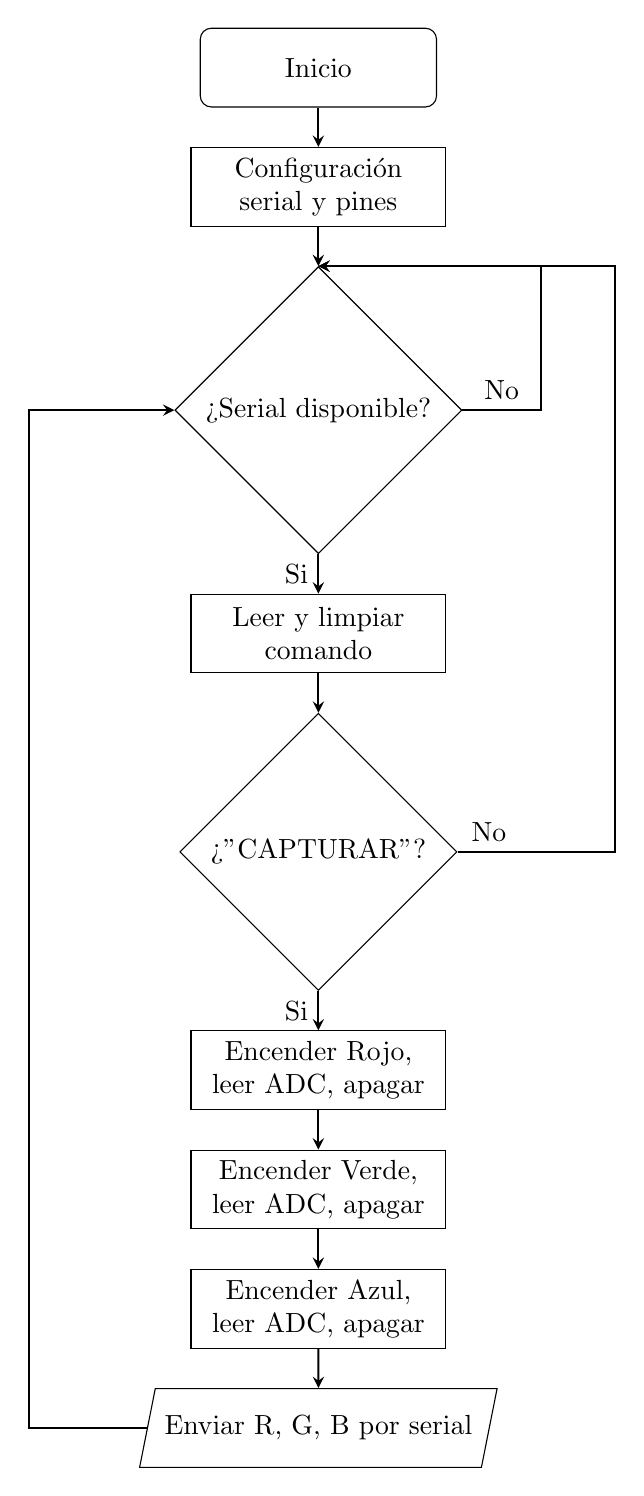
\begin{tikzpicture}[node distance=0.5cm, auto]
        % Definición de nodos (Mantenemos tus estilos)
        \node (start) [startstop] {Inicio};
        \node (pro1) [process, below=of start] {Configuración serial y pines};
        \node (dec1) [decision, below=of pro1] {¿Serial disponible?};
        \node (pro2) [process, below=of dec1] {Leer y limpiar comando};
        \node (dec2) [decision, below=of pro2] {¿"CAPTURAR"?};
        \node (pro3) [process, below=of dec2] {Encender Rojo, leer ADC, apagar};
        \node (pro4) [process, below=of pro3] {Encender Verde, leer ADC, apagar};
        \node (pro5) [process, below=of pro4] {Encender Azul, leer ADC, apagar};
        \node (out1) [io, below=of pro5] {Enviar R, G, B por serial};
        
        % --- CONEXIONES CORREGIDAS ---
        
        \draw [arrow] (start) -- (pro1);
        \draw [arrow] (pro1) -- (dec1);
        
        % 1. No Serial: Vuelve a Configuración por la derecha
        \draw [arrow] (dec1.east) -- ++(1,0) node[midway, above] {No} |- (dec1.north); 
        
        % Si Serial: Baja normal
        \draw [arrow] (dec1) -- node[anchor=east] {Si} (pro2);
        \draw [arrow] (pro2) -- (dec2);
        
        % 2. No Capturar: Vuelve a Serial disponible (Llega por ARRIBA para no solapar)
        \draw [arrow] (dec2.east) -- ++(2,0) node[pos=0.2, above] {No} |- (dec1.north);
        
        % Si Capturar: Proceso secuencial
        \draw [arrow] (dec2) -- node[anchor=east] {Si} (pro3);
        \draw [arrow] (pro3) -- (pro4);
        \draw [arrow] (pro4) -- (pro5);
        \draw [arrow] (pro5) -- (out1);
        
        % 3. Retorno final: Vuelve a Serial disponible (Llega por la IZQUIERDA)
        \draw [arrow] (out1.west) -- ++(-1.5,0) |- (dec1.west);

    \end{tikzpicture}
    }
    \caption{Diagrama de flujo del firmware de adquisición de la ESP32 (\texttt{capturar\_datos\_ESP.ino}).}
    \label{fig:diag_capturar_datos}
\end{figure}

\subsubsection{Script de Generación de Base de Datos (Python)}
Se desarrolló un script en Python utilizando la librería \texttt{pyserial} para construir un \textit{dataset} controlado \cite{ldr_14}. Este programa funciona por línea de comandos e interactúa con el usuario solicitando la etiqueta textual del color que se va a escanear. Al ingresar la etiqueta, el script envía el comando de activación a la ESP32, recibe la firma espectral (R, G, B) de 12 bits, le adjunta la etiqueta proporcionada por el usuario, para luego anexar esta fila al archivo \texttt{datos\_color.csv} (Fig. \ref{fig:diag_generar_bd}). Este proceso permitió registrar múltiples muestras por color para capturar la varianza natural del sensor.

\begin{figure}[htbp]
    \centering
    \resizebox{1\columnwidth}{!}{
    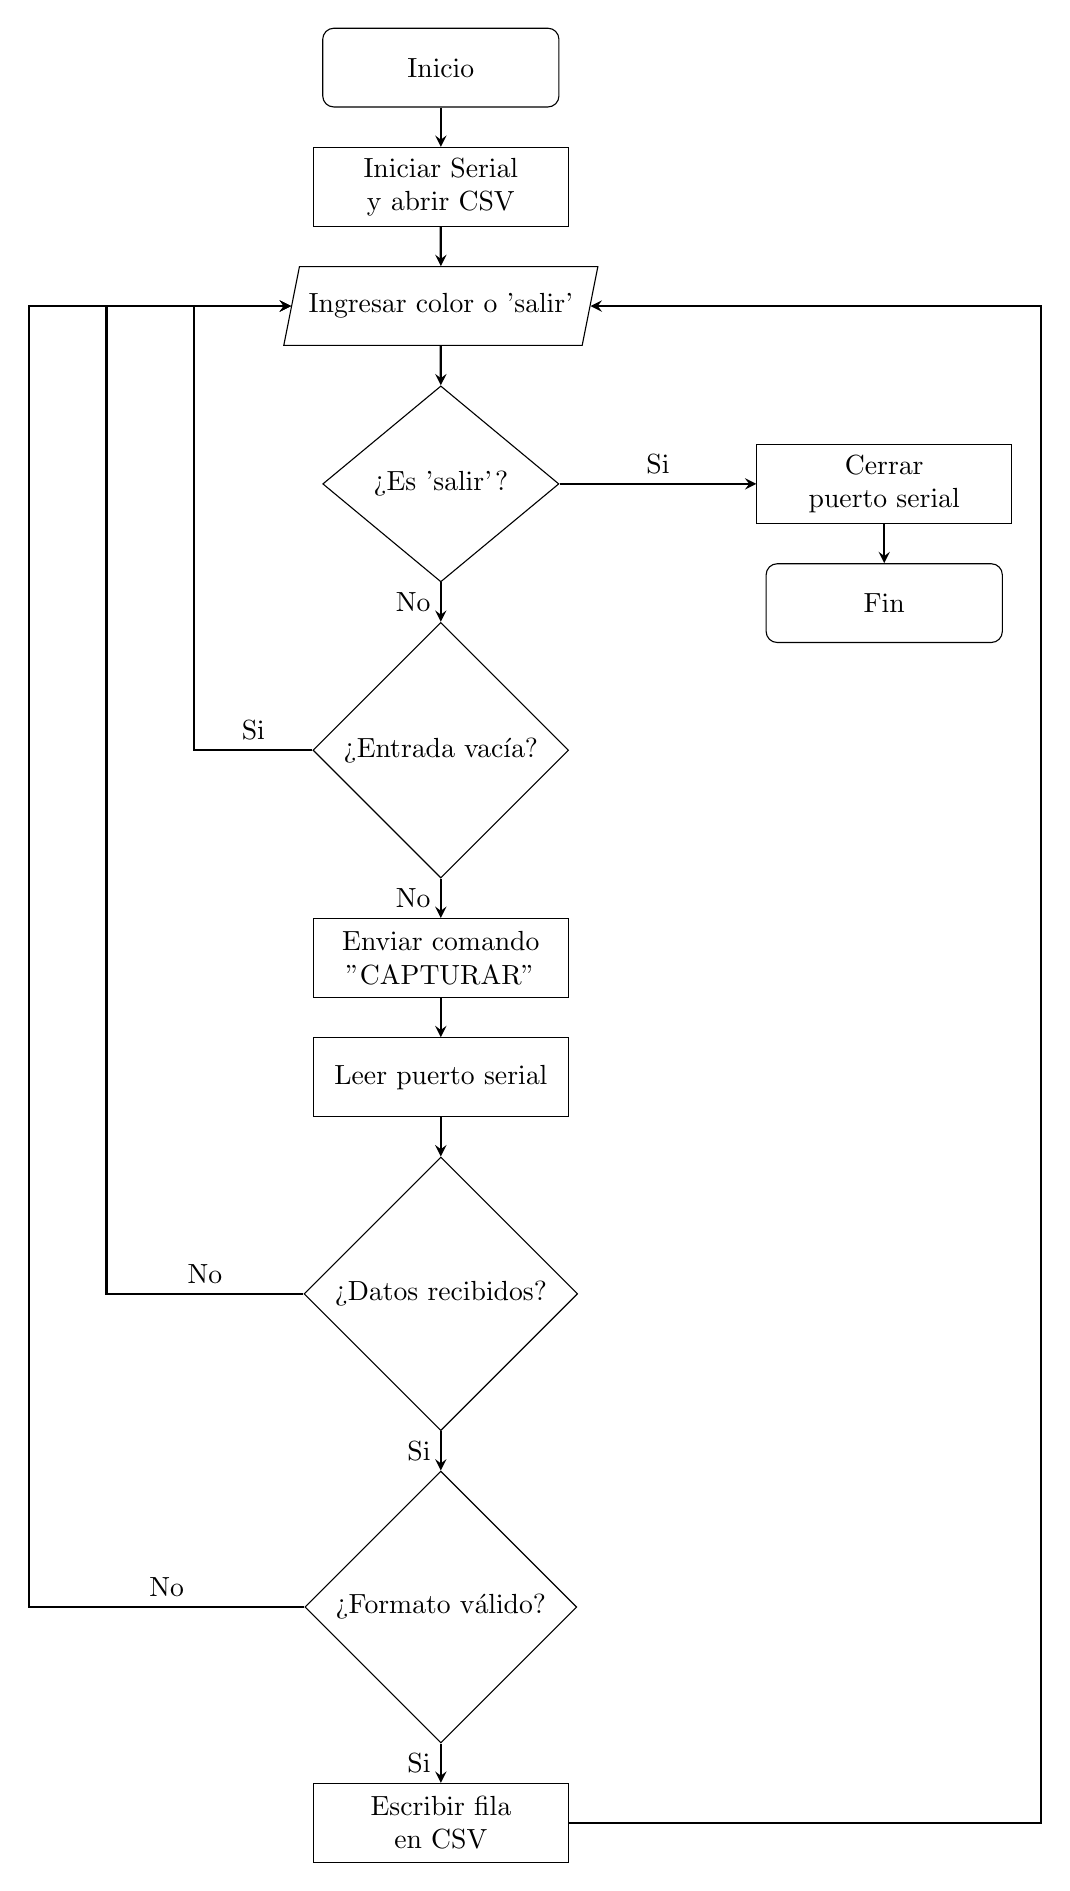
\begin{tikzpicture}[node distance=0.5cm, auto]
        
        % --- Definición de nodos ---
        \node (start) [startstop] {Inicio};
        \node (init) [process, below=of start] {Iniciar Serial y abrir CSV};
        \node (input_color) [io, below=of init] {Ingresar color o 'salir'};
        \node (dec_salir) [decision, below=of input_color] {¿Es 'salir'?};
        \node (dec_vacio) [decision, below=of dec_salir] {¿Entrada vacía?};
        \node (proc_enviar) [process, below=of dec_vacio] {Enviar comando "CAPTURAR"};
        \node (proc_leer) [process, below=of proc_enviar] {Leer puerto serial};
        \node (dec_recibido) [decision, below=of proc_leer] {¿Datos recibidos?};
        \node (dec_formato) [decision, below=of dec_recibido] {¿Formato válido?};
        \node (proc_guardar) [process, below=of dec_formato] {Escribir fila en CSV};
        
        % Nodos de salida (Ramificación a la derecha)
        \node (close) [process, right=of dec_salir, xshift=2cm] {Cerrar puerto serial};
        \node (stop) [startstop, below=of close] {Fin};

        % --- Conexiones del flujo principal (Camino de éxito) ---
        \draw [arrow] (start) -- (init);
        \draw [arrow] (init) -- (input_color);
        \draw [arrow] (input_color) -- (dec_salir);
        \draw [arrow] (dec_salir) -- node[anchor=east] {No} (dec_vacio);
        \draw [arrow] (dec_vacio) -- node[anchor=east] {No} (proc_enviar);
        \draw [arrow] (proc_enviar) -- (proc_leer);
        \draw [arrow] (proc_leer) -- (dec_recibido);
        \draw [arrow] (dec_recibido) -- node[anchor=east] {Si} (dec_formato);
        \draw [arrow] (dec_formato) -- node[anchor=east] {Si} (proc_guardar);

        % --- Conexiones de finalización (Lado Derecho) ---
        \draw [arrow] (dec_salir) -- node[anchor=south] {Si} (close);
        \draw [arrow] (close) -- (stop);

        % --- Conexiones de retorno al inicio del loop (input_color) ---
        
        % 1. Éxito: Vuelve a pedir color (Por la derecha, no se cruza porque baja más que 'close')
        \draw [arrow] (proc_guardar.east) -- ++(6,0) |- (input_color.east);

        % 2. Error/Reintento: Entrada vacía (Por la izquierda)
        \draw [arrow] (dec_vacio.west) -- ++(-1.5,0) node[midway, above] {Si} |- (input_color.west);
        
        % 3. Error/Reintento: Sin respuesta de la ESP32 (Por la izquierda, más abierto)
        \draw [arrow] (dec_recibido.west) -- ++(-2.5,0) node[midway, above] {No} |- (input_color.west);
        
        % 4. Error/Reintento: Formato incorrecto (Por la izquierda, el más abierto)
        \draw [arrow] (dec_formato.west) -- ++(-3.5,0) node[midway, above] {No} |- (input_color.west);

    \end{tikzpicture}
    }
    \caption{Diagrama de flujo del script en Python para la recolección de datos (\texttt{generar\_bd.py}).}
    \label{fig:diag_generar_bd}
\end{figure}

\subsubsection{Interfaz Gráfica y Algoritmo de Clasificación (Python y Tkinter)}
El tercer programa es el clasificador en tiempo real. Se implementó una interfaz gráfica de usuario (GUI) con \texttt{Tkinter} que permite realizar lecturas con un solo clic. El corazón de este código es su algoritmo de clasificación basado en K-Vecinos Más Cercanos (KNN con $k=1$) \cite{ldr_6}. 

Cuando la ESP32 envía una nueva lectura $(r_{cap}, g_{cap}, b_{cap})$, el algoritmo iterará sobre todos los registros $(r_{db}, g_{db}, b_{db})$ del archivo CSV calculando la distancia euclidiana tridimensional:

\begin{equation}
d = \sqrt{(r_{cap} - r_{db})^2 + (g_{cap} - g_{db})^2 + (b_{cap} - b_{db})^2}
\label{eq:dist}
\end{equation}

El sistema identifica la muestra en la base de datos que minimice esta distancia y clasifica la tarjeta actual con la etiqueta de dicho registro. Adicionalmente, el programa realiza un mapeo lineal de los valores de 12 bits (0-4095) del ADC a un formato hexadecimal de 8 bits (0-255) (Fig. \ref{fig:diag_visualizacion}) para previsualizar sintéticamente el color escaneado y el color emparejado en los lienzos (\textit{Canvas}) de la interfaz gráfica como se muestra en la figura \ref{fig:GUI}.

\begin{figure}[htbp]
    \centering
    \resizebox{0.6\columnwidth}{!}{
    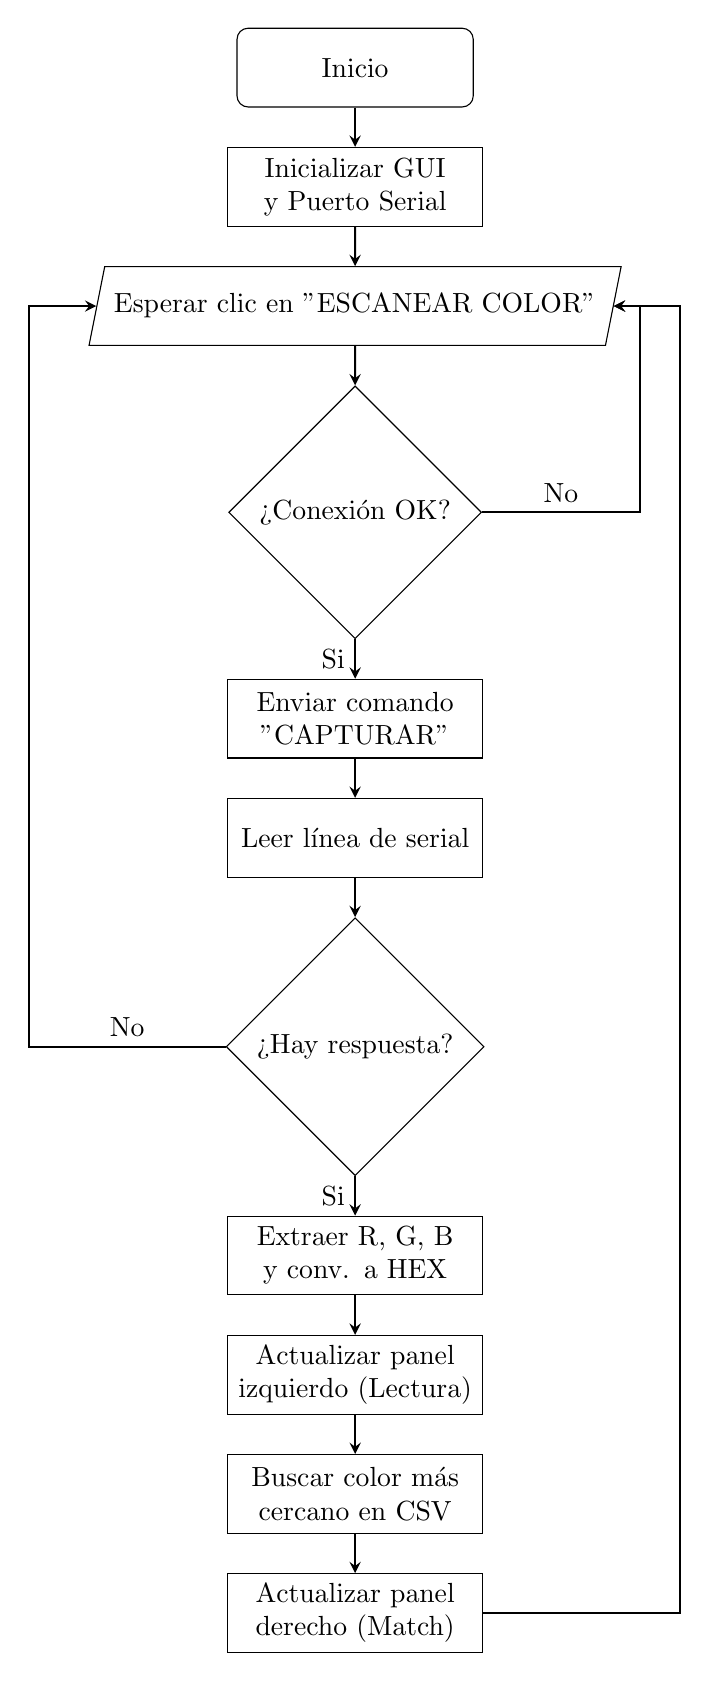
\begin{tikzpicture}[node distance=0.5cm, auto]
        
        % --- Definición de nodos ---
        \node (start) [startstop] {Inicio};
        \node (init) [process, below=of start] {Inicializar GUI y Puerto Serial};
        \node (wait) [io, below=of init] {Esperar clic en "ESCANEAR COLOR"};
        \node (dec_conn) [decision, below=of wait] {¿Conexión OK?};
        \node (send) [process, below=of dec_conn] {Enviar comando "CAPTURAR"};
        \node (read) [process, below=of send] {Leer línea de serial};
        \node (dec_resp) [decision, below=of read] {¿Hay respuesta?};
        \node (proc_parse) [process, below=of dec_resp] {Extraer R, G, B y conv. a HEX};
        \node (proc_ui1) [process, below=of proc_parse] {Actualizar panel izquierdo (Lectura)};
        \node (proc_db) [process, below=of proc_ui1] {Buscar color más cercano en CSV};
        \node (proc_ui2) [process, below=of proc_db] {Actualizar panel derecho (Match)};

        % --- Conexiones del flujo principal (Camino de éxito) ---
        \draw [arrow] (start) -- (init);
        \draw [arrow] (init) -- (wait);
        \draw [arrow] (wait) -- (dec_conn);
        
        \draw [arrow] (dec_conn) -- node[anchor=east] {Si} (send);
        \draw [arrow] (send) -- (read);
        \draw [arrow] (read) -- (dec_resp);
        
        \draw [arrow] (dec_resp) -- node[anchor=east] {Si} (proc_parse);
        \draw [arrow] (proc_parse) -- (proc_ui1);
        \draw [arrow] (proc_ui1) -- (proc_db);
        \draw [arrow] (proc_db) -- (proc_ui2);

        % --- Conexiones de retorno al estado de espera ---
        
        % 1. Éxito: Termina el proceso y vuelve a esperar otro clic (Por la derecha)
        \draw [arrow] (proc_ui2.east) -- ++(2.5,0) |- (wait.east);

        % 2. Error: No hay conexión (Por la izquierda)
        \draw [arrow] (dec_conn.east) -- ++(2,0) node[midway, above] {No} |- (wait.east);
        
        % 3. Error: Timeout / ESP32 no respondió a tiempo (Por la izquierda, más abierto)
        \draw [arrow] (dec_resp.west) -- ++(-2.5,0) node[midway, above] {No} |- (wait.west);

    \end{tikzpicture}
    }
    \caption{Diagrama de flujo de la interfaz gráfica y algoritmo de clasificación (\texttt{visualizacion.py}).}
    \label{fig:diag_visualizacion}
\end{figure}

\begin{figure}[htbp]
    \centering
    
\includegraphics[width=1\linewidth]{GUI.png}
    \caption{Interfaz gráfica del código \texttt{visualizacion.py}.}
    \label{fig:GUI}
\end{figure}

\section{Resultados y discusión}
\subsection{Resultados de la Captura de Datos}
Para evaluar la viabilidad del sistema de clasificación, se construyó una base de datos empírica (\texttt{datos\_color.csv}) capturando múltiples muestras para una variedad de colores sólidos. Con el fin de normalizar la interpretación de los datos, las lecturas originales del ADC de 12 bits (0-4095) se mapearon a un rango estándar de 8 bits (0-255). La Tabla \ref{tab:promedios_color} resume el comportamiento espectral del sensor, mostrando el valor promedio obtenido en cada canal (Rojo, Verde y Azul) para los colores analizados.

\begin{table}[htbp]
    \centering
    \caption{Valores promedio de reflectancia escalados al rango 0-255 para cada color.}
    \begin{tabular}{|l|c|c|c|}
        \hline
        \makecell{Color\\Escaneado} & 
        \makecell{Canal\\Rojo ($R$)} & 
        \makecell{Canal\\Verde ($G$)} & 
        \makecell{Canal\\Azul ($B$)}  \\
        \hline
        Amarillo   & 220 & 206 & 50  \\
        Azul       & 45  & 60  & 226 \\
        Blanco     & 237 & 234 & 242 \\
        Celeste    & 111 & 201 & 237 \\
        Cian       & 53  & 199 & 206 \\
        Gris       & 125 & 125 & 123 \\
        Lima       & 112 & 223 & 24  \\
        Magenta    & 212 & 48  & 217 \\
        Marron     & 74  & 50  & 32  \\
        Naranja    & 226 & 112 & 37  \\
        Negro      & 9   & 10  & 7   \\
        Oliva      & 75  & 87  & 21  \\
        Oro        & 188 & 161 & 25  \\
        Purpura    & 125 & 23  & 155 \\
        Rojo       & 216 & 51  & 47  \\
        Rosa       & 238 & 138 & 155 \\
        Salmon     & 218 & 94  & 75  \\
        Turquesa   & 24  & 199 & 188 \\
        Verde      & 58  & 193 & 56  \\
        Violeta    & 92  & 31  & 188 \\
        \hline
    \end{tabular}
    \label{tab:promedios_color}
\end{table}



Como se observa en la tabla \ref{tab:promedios_color}, el diseño de hardware logró un aislamiento óptico efectivo y una respuesta coherente con la teoría del color. Por ejemplo, al exponer el sensor a la tarjeta roja, la reflectancia máxima se da cuando el LED ilumina en el canal rojo ($R \approx 215$), mientras que la tarjeta absorbe casi por completo las longitudes de onda del verde y el azul, resultando en lecturas significativamente menores ($G \approx 51$, $B \approx 47$). 

Este comportamiento se repite consistentemente en los colores primarios luz (Verde y Azul). Además, los colores compuestos o secundarios mostraron firmas espectrales híbridas muy claras. El color Oro, por ejemplo, refleja altos niveles tanto de la luz roja como de la verde ($R \approx 187$, $G \approx 161$), pero absorbe casi en su totalidad el azul ($B \approx 25$). El color Turquesa refleja fuertemente el verde y el azul ($G \approx 196, B \approx 184$), absorbiendo el rojo, mientras que el Violeta refleja el azul y moderadamente el rojo ($B \approx 187, R \approx 92$), absorbiendo el verde.

Estos valores triestímulo demuestran que la combinación de la fotorresistencia y la fuente de iluminación secuencial RGB es capaz de generar coordenadas tridimensionales $(R, G, B)$ únicas para cada pigmento físico. La separación espacial de estas coordenadas en la base de datos es lo que permite que el algoritmo de distancia euclidiana (\ref{eq:dist}) ejecutado en la interfaz de Python logre emparejar muestras en tiempo real con un alto grado de precisión.

\subsection{Análisis del Sistema y Discusión}

El éxito del clasificador de color no radica únicamente en la fidelidad de la captura de datos del hardware, sino en el procesamiento algorítmico posterior. La implementación de la distancia euclidiana (ecuación \ref{eq:dist}) como método de clasificación (un enfoque basado en el algoritmo de los $k$-vecinos más cercanos, con $k=1$) demostró ser altamente eficiente. 

Al tratar las lecturas de los canales capturados como coordenadas espaciales $(R, G, B)$ dentro de un espacio tridimensional, el script de Python logra emparejar la muestra actual con el registro histórico más cercano evaluando la mínima distancia $d$.

Dado que los valores espectrales de cada color se agrupan en clústeres bien definidos y alejados entre sí (como se evidenció en la tabla \ref{tab:promedios_color}), el margen de error del sistema es prácticamente nulo al evaluar tonos sólidos y contrastantes. El sistema mapea correctamente la firma óptica del objeto y la correlaciona con la base de datos en tiempo real.

\subsubsection*{Limitaciones y Fuentes de Error}
A pesar de la robustez lógica del software, el análisis empírico durante las pruebas reveló que el sistema es altamente dependiente de las condiciones físicas del entorno. Las principales limitaciones identificadas fueron:

\begin{itemize}
    \item Interferencia de luz ambiental: El fotorresistor (LDR) es extremadamente sensible. Aunque la resistencia del divisor de tensión de $10\text{ k}\Omega$ optimiza el rango dinámico del ADC, cualquier filtración de luz externa sobre la superficie de prueba suma un "offset" a la reflectancia leída. Esto desplaza las coordenadas $(R, G, B)$ capturadas, lo que puede derivar en clasificaciones erróneas o falsos positivos \cite{ldr_7}.
    
    \item Sensibilidad a la distancia focal: Debido a la ley de la inversa del cuadrado para la intensidad luminosa, pequeñas variaciones en la distancia entre los LEDs, el sensor y la tarjeta de color provocan fluctuaciones masivas en los valores del ADC. Para que la base de datos sea válida, la distancia de escaneo debe mantenerse estandarizada e invariable \cite{ldr_8}.
    
    \item Latencia del LDR (Efecto memoria): El sulfuro de cadmio (CdS) del que están compuestos los fotorresistores presenta una respuesta temporal asimétrica, tardando más en adaptarse a la oscuridad que a la luz \cite{ldr_9}. Los tiempos de espera de 200 milisegundos (\texttt{delay(200)}) programados en el firmware de la ESP32 entre cada encendido de color resultaron ser un compromiso crítico y necesario para permitir que la resistencia del sensor se estabilizara y evitar una superposición residual de lecturas entre canales adyacentes.
\end{itemize}

En síntesis, la arquitectura del sistema embebido junto con la interfaz gráfica proporciona una herramienta educativa y funcional excelente. No obstante, para llevar este principio a una aplicación industrial, sería imperativo sustituir el módulo abierto por una cámara oscura hermética que aisle el entorno de medición.

\section{Conclusiones}

Tras el diseño, montaje y puesta a prueba del sensor optoelectrónico de reflectancia, se extraen las siguientes conclusiones respecto al desempeño del sistema y los objetivos planteados:

\begin{itemize}
    \item Validación del principio físico: Se comprobó exitosamente que la combinación de un LED RGB secuencial y un fotorresistor (LDR) en un divisor de tensión es un método válido y de bajo costo para extraer firmas espectrales tridimensionales $(R, G, B)$ de superficies opacas, permitiendo al algoritmo de distancia euclidiana (ecuación \ref{eq:dist}) clasificar colores básicos con un alto índice de acierto.

    \item Error e incertidumbre en las mediciones: Se evidenció un margen de error significativo en las lecturas analógicas capturadas por la ESP32. Aunque el microcontrolador posee un ADC de 12 bits de alta precisión, el error proviene de la naturaleza física del LDR y del entorno. Las ligeras variaciones en la distancia focal (incluso del orden de milímetros al colocar las tarjetas), la contaminación lumínica del ambiente y el ruido térmico del circuito provocan que un mismo color arroje valores fluctuantes en diferentes escaneos \cite{ldr_10}. Esta varianza genera "nubes de incertidumbre" o dispersión en los datos para cada color almacenado en el archivo CSV.

    \item Incumplimiento del objetivo de 50 colores: El objetivo inicial del laboratorio, consistente en detectar y clasificar la mayor cantidad posible de tarjetas, fijando una meta de 50 colores diferentes, no pudo ser alcanzado. El sistema demostró ser estable únicamente para un número reducido de tonos altamente contrastantes (colores primarios y algunos secundarios muy definidos).

    \item Justificación de la limitación (Baja resolución espectral): La incapacidad de clasificar 50 colores radica en la física del hardware utilizado. Un LED RGB emite luz en tres bandas espectrales muy anchas. Al intentar escanear una paleta extensa (por ejemplo, introduciendo tonos como salmón, coral, naranja y rojo claro), el LDR arrojaba firmas $(R, G, B)$ virtualmente idénticas para todos ellos.
    
    Al combinarse esta similitud espectral con el error de medición previamente mencionado, los clústeres de datos se superponían geométricamente en el espacio tridimensional evaluado por el algoritmo en Python. En consecuencia, la distancia euclidiana perdía su eficacia, generando constantes falsos positivos y emparejamientos erróneos al no poder discernir si la variación en la lectura se debía a un cambio real de color o simplemente al ruido del sensor \cite{ldr_10}.

    \item Trabajo futuro: Se concluye que, si bien este montaje es excelente con fines pedagógicos para comprender la optoelectrónica básica y el procesamiento de señales, escalar el proyecto a una discriminación fina de 50 o más colores requiere hardware especializado. Para trabajos futuros, se recomienda la transición a sensores de color digitales integrados (como el TCS3200 o el AS7341), los cuales cuentan con matrices de fotodiodos con filtros ópticos de banda estrecha e inmunidad al ruido ambiental, garantizando la repetibilidad y resolución necesarias para una colorimetría precisa.
\end{itemize}

\bibliographystyle{IEEEtran}
\bibliography{IEEEabrv,biblio_traps_dynamics}

\end{document}